\subsection{Apache Airflow™}
Apache Airflow™ stands as an open-source platform designed to manage data flow
within systems associated with data. In the face of the escalating challenge of
data pipeline management, Airflow emerges as a comprehensive solution,
automating and optimizing data-related workflows effectively \cite{airflow}.

Airflow not only aids in defining and managing the start and end times of each
data pipeline but also provides precise and detailed monitoring of the results
of each task. This becomes particularly crucial when ensuring the integrity and
reliability of the processed data.

With the ability to discern complex relationships between tasks through the
Directed Acyclic Graph (DAG) model, Airflow empowers administrators with tighter
control and flexibility in handling workflow processes. Its robust integration
with logging systems facilitates detailed activity tracking, assisting in issue
resolution and ensuring that every process aligns with expectations.

Simultaneously, the scheduling flexibility makes Airflow an excellent tool for
time and resource management. Its strong integration with various data sources
and extensibility through plugins allows Airflow to meet diverse needs in data
processing and task automation.

Apache Airflow not only delivers robust performance but also brings flexibility
and optimal technical features to data processing workflows. With its time
management capabilities, powerful logging integration, scheduling flexibility,
and scalability, Airflow stands as the top choice for enhancing performance and
control in data processing workflows.

\subsection{Kubernetes}
Kubernetes, an open-source system for managing and deploying highly flexible
applications in cloud and data center environments, has evolved into one of the
most widely adopted tools in the field of Information Technology \cite{k8s-doc}.
Originally developed by Google and later transferred to the Cloud Native
Computing Foundation (CNCF), Kubernetes aims to automate the deployment,
scaling, and management of containerized applications, alleviating the burden on
developers and system administrators. The platform offers a unified foundation
for deploying, scaling, and managing containerized applications across multiple
servers.

Kubernetes operates based on key concepts such as Pods, Services, ReplicaSets,
and various other abstractions, creating a flexible environment for application
deployment and management. This fosters an environment where developers can
easily build applications, and system administrators can efficiently maintain
them.

Beyond supporting traditional deployment models, Kubernetes paves the way for
innovative strategies like Continuous Deployment (CD) and Microservices. With
the ability to automate many aspects of the development and deployment process,
Kubernetes plays a crucial role in constructing and sustaining complex,
flexible, and scalable systems.

\subsubsection*{Kubernetes Components}
Introducing essential concepts for managing and deploying applications,
Kubernetes provides an effective and flexible environment. The main components
of Kubernetes include Pod, ReplicaSet, Deployment, and Service.

\begin{figure}[H]
    \centering
    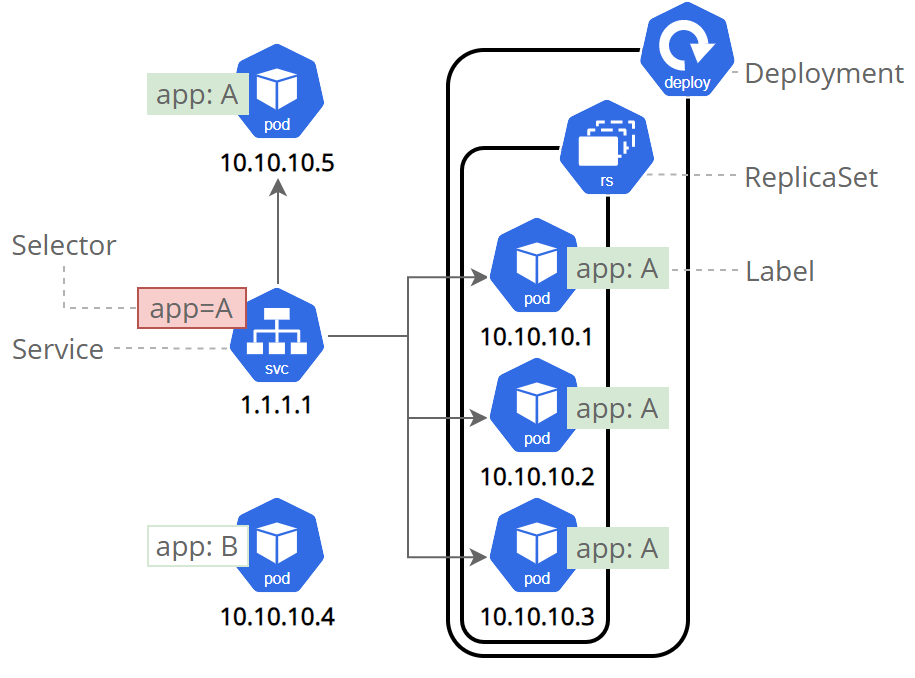
\includegraphics[width=0.75\linewidth]{Images/3.4-k8s-comps.png}
    \caption{Overview of Kubernetes Components - Kubernetes}
    \label{fig:k8s-comps}
\end{figure}

In Kubernetes, a \textbf{Pod} serves as the fundamental unit, representing a
collection of containers that share a common workspace. Within the same Pod,
containers collaborate by sharing network and storage resources, fostering
interaction and enabling the construction of intricate applications.

The \textbf{ReplicaSet}, a crucial resource in Kubernetes, ensures a designated
number of Pods operate in a specified manner. In the event of a Pod failure or
shutdown, the ReplicaSet automatically initiates the creation of a new Pod to
replace it. This mechanism ensures the application's stable state by
guaranteeing a defined number of Pods are consistently operational.

For managing the deployment and updating processes of applications,
\textbf{Deployment} is a key component in Kubernetes. It articulates the desired
state of the application and orchestrates the updating of the ReplicaSet to
achieve that state. Deployment provides versatile management capabilities,
facilitating the deployment of new versions, rollbacks, and updates without
disrupting the service.

The \textbf{Service} resource in Kubernetes furnishes an HTTP port to Pods,
generating a unique IP address and DNS name for a cluster of Pods. This enables
seamless communication among applications within the cluster and with external
environments. Service effectively simplifies the intricacies of handling
multiple Pods and IP addresses, offering a straightforward means of accessing
services within the Kubernetes environment.

Typically, large-scale systems leverage Kubernetes in their software development
and deployment processes. This adoption brings several advantages, including
efficient resource management and self-recovery capabilities. Kubernetes
optimizes resource utilization, ensuring optimal performance and reducing waste.
Additionally, it automatically addresses issues during operations, enhancing
high availability.

However, the technology is not without its challenges, including a steep
learning curve for beginners. Mastery of diverse knowledge areas such as
computer networking and containerization is necessary. Moreover, deploying and
maintaining Kubernetes demands significant resources, both in terms of personnel
and hardware, particularly for smaller organizations.

\subsubsection*{High Availability in Kubernetes}
High Availability is a crucial factor in the success of any system. In
Kubernetes, High Availability is achieved through the combination of several
features, including self-healing, load balancing, and auto-scaling.

First, Kubernetes uses \textbf{Deployment}, a type of \textbf{Controller} for
managing replicas. Through Deployment, we can easily perform horizontal scaling,
which is the process of increasing the number of replicas of a Pod. This
mechanism ensures that the application can handle numerous requests without
compromising performance. Moreover, in case of a Pod failure, a Deployment makes
sure that a new Pod is created to replace it, ensuring the amounts of predefined
replicas is always maintained.

At network layers, Kubernetes uses \textbf{Service} for communication between
various components within or outside the cluster. Instead of directly accessing
Pods, other components can access Services, which will redirect the request to
the appropriate Pod. When Pods are replaced, the Service will automatically
update the routing rules to ensure the request is sent to the correct Pod.
Outside the cluster, Kubernetes also uses \textbf{Ingress} to manage external
access to Services. Instead of specifying the direct node IP address, Clients
can abstract it by using only the URL or hostname.

Finally, at the storage level, Kubernetes provides Persistent Volumes. By doing
so, applications can be agnostic to the underlying storage infrastructure. This
allows for easier management and scaling of storage resources. Not only that,
depending on the provided \textbf{Storage Class}, Kubernetes makes sure that the
data is replicated to multiple nodes, ensuring data availability in case of node
failure.

To summarize, Kubernetes provides a robust set of features to ensure High
Availability. By leveraging these features, we can build a highly available
system that can scale with our load, while also being resilient to failures.

\subsection{LROSE}
LROSE (Lidar Radar Open Software Environment) is a project supported by the
National Science Foundation (NSF) with the goal of developing common software
for the Lidar, Radar, and Profiler community. The project operates based on the
principles of collaboration and open source. The core software package of LROSE
is a collaborative effort between Colorado State University (CSU) and the Earth
Observing Laboratory (EOL) at the National Center for Atmospheric Research
(NCAR) \cite{lrose}.

Originating from the need for a unified software environment for processing
Lidar and Radar data in atmospheric science research \cite{lrose}, the project
addresses complexities related to integrating data from various observation
platforms, including Lidar, Radar, and Profiler. These components are designed
to meet the specific needs of meteorologists and researchers working with remote
sensor data.

LROSE is widely used in meteorological research, including studies related to
cloud and precipitation processes, boundary layer dynamics, and other
meteorological phenomena. The software supports the analysis of observation data
collected from ground-based tools such as Lidar and Radar. LROSE seamlessly
integrates with a variety of model and atmospheric analysis tools to optimize
its capabilities. Researchers often integrate LROSE into numerical weather
prediction models as well as other data assimilation techniques, creating a
flexible and powerful system.

\begin{figure}[H]
    \centering
    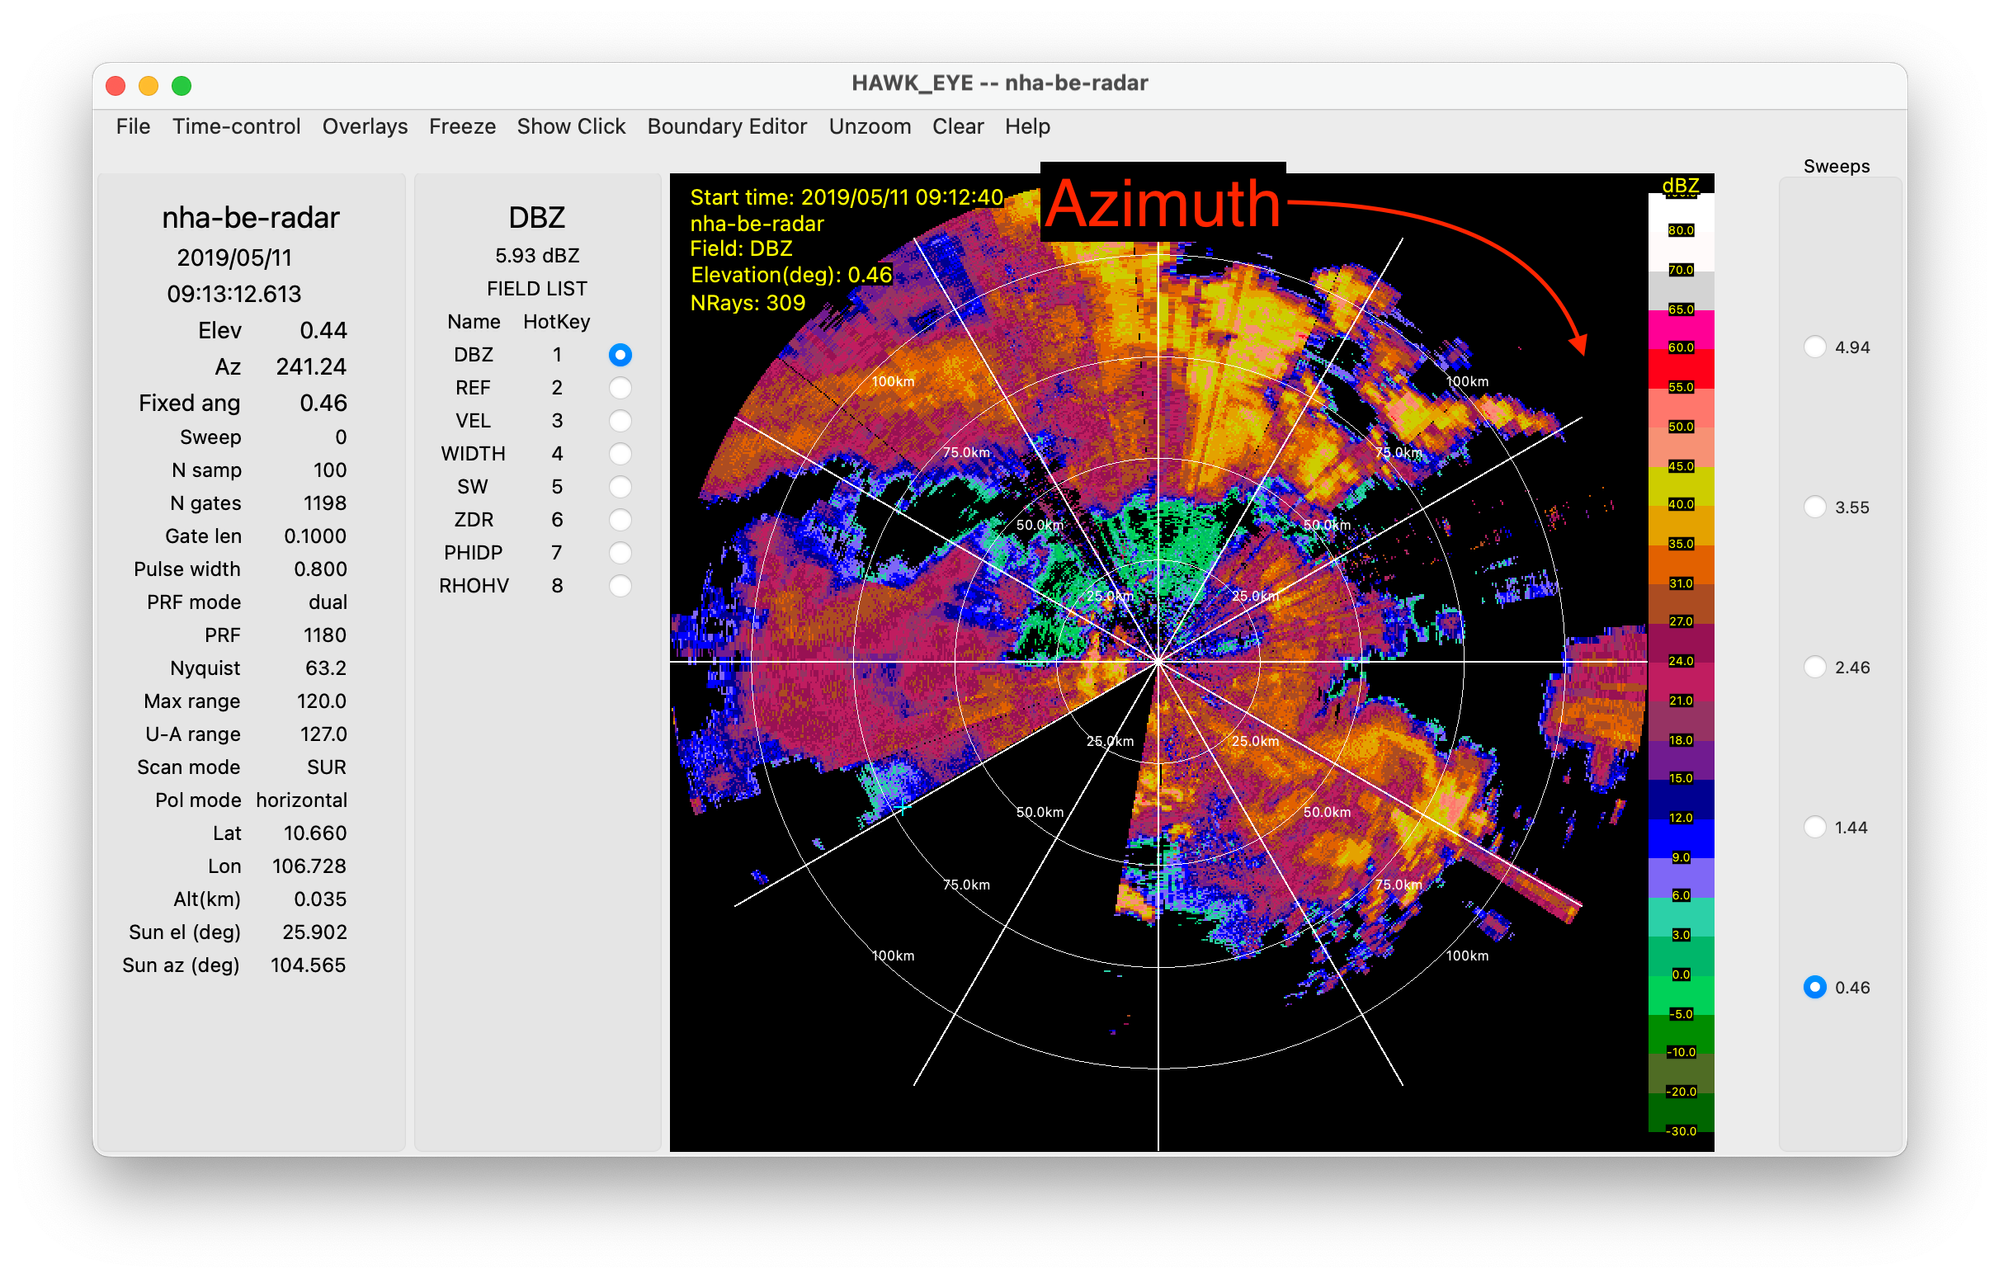
\includegraphics[width=0.8\linewidth]{Images/3.5-hawk-eye.png}
    \caption{Hawk Eye, Lidar and Radar visualization tool of LROSE}
    \label{fig:hawk-eye}
\end{figure}

The project actively encourages participation from a large scientific community,
promoting the exchange of ideas, algorithms, and improvements for the software.
Regular updates and contributions from users contribute to the continuous
development and refinement of LROSE.

% =================================================================================
% Py-ART
% =================================================================================

\subsection{Py-ART}
In the realm of meteorology, weather radar plays a crucial role in understanding
and forecasting precipitation, cloud cover, and other atmospheric phenomena.
Extracting meaningful information from this data requires specialized tools and
techniques. Py-ART (the Python ARM Radar Toolkit) is an open-source Python
library designed specifically for working with weather radar data.

Developed by the Atmospheric Radiation Measurement (ARM) Climate Research
Facility, Py-ART offers a comprehensive suite of algorithms and utilities for
researchers and atmospheric scientists. However, its user-friendly design and
extensive functionalities make it valuable for anyone working with weather radar
data, from meteorologists to students.

\subsubsection*{Core functionalities}
Py-ART transcends its role as a simple data repository. It empowers users with a
comprehensive suite of functionalities, transforming raw weather radar data into
meaningful insights.  At its core, Py-ART offers a robust toolbox for data
manipulation, analysis, and visualization, catering to the diverse needs of
meteorologists, researchers, and anyone working with weather radar information.

The journey begins with seamless data access. Py-ART supports a wide range of
file formats commonly used in atmospheric research. This versatility allows
users to import data from various sources, eliminating compatibility hurdles and
streamlining the workflow. Once the data is loaded, Py-ART's processing
capabilities come into play. Real-world radar measurements are not without
imperfections. Signal attenuation, caused by factors like distance and
intervening obstacles, weakens the returning signal. Py-ART provides algorithms
to correct for this attenuation, ensuring the accuracy of the retrieved
information. Furthermore, raw radar data often contains noise – unwanted
electrical disturbances that can distort the signal. Py-ART offers a variety of
filtering techniques to remove this noise, resulting in a cleaner and more
reliable dataset. Calibration, a crucial step in ensuring data integrity, is
also made possible by Py-ART. By applying calibration techniques, users can
account for systematic biases inherent in the radar system, leading to more
precise measurements.

Once the data is cleaned and processed, Py-ART shines in its ability to
visualize and analyze this information. It seamlessly integrates with popular
scientific Python libraries like Matplotlib. This powerful combination allows
users to create informative and visually compelling representations of the data.
Imagine generating high-resolution reflectivity maps that paint a vivid picture
of precipitation intensity across a region. Py-ART facilitates this by
converting reflectivity data into maps, allowing for easy identification of
areas with heavy rain or snowfall.  Beyond maps, Py-ART enables the creation of
vertical profiles, which depict how reflectivity and other parameters vary with
altitude. This provides a detailed understanding of the vertical structure of
storms and precipitation events. Analyzing these visualizations in conjunction
with environmental data, which Py-ART can also incorporate, allows researchers
to delve deeper into the atmospheric processes at play.

Py-ART's functionalities extend beyond basic visualization. It offers advanced
analysis tools for tasks like feature detection and storm tracking. Imagine
automatically identifying and tracking the movement of severe weather features
like hailstorms or tornadoes within radar data. Py-ART's algorithms can
accomplish this, providing crucial information for issuing timely weather
warnings and protecting lives.  Perhaps the most impactful functionality lies in
quantitative precipitation estimation (QPE). By analyzing radar data and
incorporating environmental factors, Py-ART can estimate the amount of
precipitation that has fallen over a specific area. This information is
invaluable for flood forecasting, water resource management, and understanding
overall precipitation patterns.

\subsubsection*{Benefits}
Py-ART offers a range of benefits for working with weather radar data, making it
a compelling choice for meteorologists and atmospheric scientists alike.
Firstly, Py-ART is open-source and freely available, allowing anyone to access,
download, and modify its code. This fosters collaboration and innovation within
the atmospheric science community, as researchers can contribute improvements
and share their work with others.

Additionally, Py-ART boasts cross-platform compatibility, functioning seamlessly
on various operating systems including Windows, macOS, and Linux. This ensures
wider accessibility and flexibility for users across different computing
environments.

The modular design of Py-ART is another key advantage, allowing users to
leverage specific functionalities they need for their radar data processing
tasks. This modular approach enhances efficiency and adaptability, as users can
tailor their workflow to suit their requirements.

Moreover, Py-ART provides extensive documentation and a rich collection of
examples, which serve to ease the learning curve for new users. The availability
of comprehensive resources empowers users to quickly familiarize themselves with
the library's capabilities and effectively utilize its features for their
research or operational needs.

% =================================================================================
% Compare LROSE and PY-ART
% =================================================================================

\subsection{Comparing between the tools of LROSE and PyART for Meteorology Data Processing}
In meteorology, data processing is essential for interpreting and understanding
atmospheric phenomena. While both tools offer robust functionalities for radar
and lidar data processing, PyART stands out due to its seamless integration with
Python, making it particularly powerful for researchers and developers who
leverage Python's extensive scientific ecosystem. This section compares these
two tools across several dimensions: functionality, ease of use, extensibility,
community support, and performance, with a focus on PyART's advantages.

\subsubsection*{Functionality}
PyART offers a comprehensive suite of tools and features for radar data
analysis. It supports data input and output in multiple formats, including
NetCDF, HDF5, and MDV, ensuring compatibility with various data sources. In
terms of processing algorithms, PyART provides robust options for data
correction such as dealiasing and attenuation correction, alongside filtering
and moment calculation. For visualization, PyART integrates seamlessly with
Matplotlib, enabling users to create detailed 2D and 3D visual representations
like PPI (Plan Position Indicator) and RHI (Range Height Indicator) plots.
Furthermore, PyART is built on the SciPy ecosystem, which facilitates easy
integration with other Python scientific libraries such as NumPy, Pandas, and
Scikit-learn, thus significantly enhancing its analytical capabilities.

On the other hand, LROSE-Core is also an extensive suite aimed at standardizing
and enhancing radar and lidar data processing capabilities. Developed as an
open-source initiative, it emphasizes interoperability and advanced processing
techniques. The suite supports a wide range of radar and lidar data formats,
including proprietary ones, making it highly versatile. LROSE-Core includes
sophisticated signal processing algorithms such as dual-polarization processing,
clutter filtering, and Doppler velocity analysis. For visualization, it offers
advanced tools through its HawkEye and CIDD applications, which provide
interactive and customizable plotting capabilities. Additionally, the toolset is
designed to handle real-time data processing, which is crucial for operational
radar networks.

\subsubsection*{Ease of Use - Learning Curve}
PyART is designed with simplicity in mind, making it accessible to users with
basic programming knowledge. The API is well-documented, and the library
includes numerous examples and tutorials. Its seamless integration with Python's
scientific stack (NumPy, XArray, and Matplotlib, ...) makes it a natural choice
for researchers already familiar with these tools. Python's ease of use and
readability further enhance PyART's appeal, allowing users to quickly prototype
and deploy analysis workflows.

LROSE-Core, while powerful, has a steeper learning curve compared to PyART. It
requires a more in-depth understanding of radar and lidar data processing
principles. The installation process can be more complex, especially for users
unfamiliar with building software from source. However, the detailed
documentation and active community support can help mitigate these challenges.

\subsubsection*{Extensibility}
PyART's modular design makes it highly extensible. Users can easily incorporate
their own algorithms or modify existing ones. Its reliance on Python ensures
that it can leverage the extensive range of available libraries for additional
functionality. This extensibility makes PyART particularly powerful, as users
can integrate machine learning libraries such as TensorFlow or Scikit-learn to
develop advanced predictive models directly within their radar data processing
workflows.

LROSE-Core is also designed for extensibility, with a focus on providing a
comprehensive platform for radar and lidar data processing. Its open-source
nature allows users to contribute new algorithms and features. However,
extending LROSE-Core may require more specialized knowledge in C++ and
radar/lidar processing techniques, potentially limiting its accessibility
compared to PyART.

% =================================================================================
% ASP.NET
% =================================================================================

\subsection{ASP.NET Core}
ASP.NET Core is a free, cross-platform, open-source framework for building
modern, cloud-based, internet-connected applications. It is particularly
well-suited for developing API servers that need to interact with databases,
thanks to its robust set of features, high performance, and strong community
support.

There are many reasons to believe that ASP.NET and C\# can be a good candidate
for building server in managing an integrated database system. The following
sections explain some key features that Microsoft and this ecosystem provides
when constructing the system.

\subsubsection*{Cross-Platform Support}
ASP.NET Core distinguishes itself through its remarkable cross-platform
compatibility, heralding a paradigm shift wherein applications developed on this
framework can seamlessly traverse the disparate terrains of Windows, Linux, and
macOS environments. This intrinsic flexibility underscores the platform's
adaptability to diverse deployment scenarios, be it the precincts of a localized
server, the ethereal expanse of a cloud platform, or the nuanced amalgam of a
hybrid setup. Such versatility empowers developers with the autonomy to
cherry-pick the operating system that resonates most harmoniously with the
exigencies of their deployment milieu, thereby engendering a milieu of
operational fluidity and infrastructural resilience.

\subsubsection*{Robust Security Features}
Security, an ever-pressing concern in the digital milieu, assumes paramount
significance in the realm of web applications, particularly those enmeshed
within the labyrinthine landscapes of database interactions. ASP.NET Core,
cognizant of this imperative, fortifies its arsenal with a plethora of built-in
mechanisms geared towards safeguarding the sanctity of data transactions. It
proffers native support for industry-standard authentication protocols and a
panoply of security features engineered to combat the insidious machinations of
common cyber threats, including but not limited to Cross-Site Scripting (XSS)
and Cross-Site Request Forgery (CSRF). Augmenting its robust security posture
are provisions for multi-factor authentication and seamless integration with
external authentication providers such as Google and Facebook, thereby
delineating a formidable bulwark against the incursions of malevolent actors.

\subsubsection*{Rich Ecosystem and Tooling}
At the heart of ASP.NET Core beats the pulse of the expansive .NET ecosystem, a
sprawling tapestry interwoven with a myriad of libraries, tools, and frameworks.
Foremost among these is Entity Framework Core (EF Core), a venerable
Object-Relational Mapper (ORM) that bestows upon developers an intuitive conduit
for data access and manipulation. Renowned for its versatility, EF Core extends
its embrace to a diverse array of database platforms, including but not limited
to SQL Server, SQLite, PostgreSQL, and MySQL, thereby furnishing developers with
the wherewithal to navigate the complex terrain of database interactions with
consummate ease and finesse.

% =================================================================================
% MinIO
% =================================================================================

\subsection{MinIO}
MinIO is an open-source, high-performance, distributed object storage system. It
is designed to be fully compatible with the Amazon S3 API, which makes it an
attractive option for developers and organizations looking to deploy scalable
and cost-effective storage solutions. MinIO's simplicity, speed, and scalability
make it suitable for a wide range of applications, from private cloud
infrastructures to data lakes and large-scale data processing environments.

\subsubsection*{S3 Compatibility and Interoperability}
A salient hallmark of MinIO lies in its comprehensive compatibility with the
Amazon S3 Application Programming Interface (API), a feature that bestows upon
it the mantle of interoperability with a plethora of applications tailored for
Amazon S3. This alignment with the S3 API translates into a seamless interplay
between MinIO and applications engineered for Amazon S3, obviating the need for
any modifications or adaptations. Furthermore, this compatibility extends across
a gamut of S3 functionalities, including but not limited to bucket policies,
multipart uploads, and the generation of presigned URLs, thereby positioning
MinIO as a compelling substitute for S3 across manifold scenarios.

\subsubsection*{High Performance and Scalability}
At the heart of MinIO's allure lies its relentless pursuit of high performance
and scalability, traits that are quintessential in navigating the exigencies of
modern data ecosystems. Engineered with a laser focus on throughput and
scalability, MinIO boasts the capability to seamlessly accommodate prodigious
volumes of data with unparalleled efficiency. Leveraging a suite of advanced
technologies, including erasure coding, bit-rot protection, and data
compression, MinIO stands poised to cater to the exacting demands levied by
high-stakes domains such as big data analytics and machine learning workloads,
positioning itself as a stalwart guardian of performance and reliability.

\subsubsection*{Security, Flexibility, and Ease of Use}
Ensuring the sanctity of data integrity, MinIO espouses a multifaceted approach
towards fortifying its security posture. Embracing server-side encryption as a
cornerstone, MinIO ensures that data remains impervious to the predations of
malevolent actors even when at rest. Moreover, bolstering its security
repertoire is the seamless integration of Transport Layer Security (TLS),
imbuing data in transit with an impenetrable cloak of encryption. Augmenting its
security credentials are robust access control mechanisms, including the
granular delineations afforded by Identity and Access Management (IAM) policies,
thereby empowering administrators with fine-grained control over data access and
manipulation. Furthermore, MinIO's minimalist design ethos renders it eminently
facile to install and manage, underscored by an intuitive web-based management
console and a potent command-line interface (CLI) replete with scripting
capabilities, thus ensuring a seamless fusion of sophistication and
user-friendliness in the realm of storage resource management.
